\documentclass{report}

\usepackage{graphicx}
\usepackage{caption}
\usepackage{subcaption}
\usepackage{amsmath}
\usepackage{amsfonts}
\captionsetup{justification=centerlast, margin=0.5cm}
\usepackage{verbatim}

\begin{document}

\chapter{Layout extraction by Maximal White Rectangle analysis.}

\section{Approach and Purpose}
% Where it comes from
The Maximal White Rectangles (MWR) approach for document layout analysis was developed by Henri S. Baird in the 90s. With recent dramatic
improvements in computing power, this technique formerly either very constrained or very slow is now achievable for full scale 150 to
300 dpi binarized documents.\\

The idea of MWR analysis comes from a global-to-local, non-backtracking document analysis approach matching the implicit approach of a human
reader. Indeed, the eye is first attracted to important white spacing from which we deduce the reading order. e.g first the margins, then isolate
the title, separate the columns of text, then the paragraph boundaries, etc. Similarly, the MWR algorithm enumerates all the maximum (by inclusion
order) empty rectangles, in a document image, and outputs them sorted by an area-based metric.\\

From that point, we are to select a given percentile of the highest-scoring MWRs, which reunion creates a template of empty zones in the original
images (see figure \ref{MWRoverlayEx}). The remaining area uncovered by selected MWRs is separated in connected components which are likely
to correspond to logical blocks in the document, given that they are surrounded by large empty areas but do not contains such large white areas.\\

The purpose of the MWR in this context is to use this overlay, to further on use the relative positions of the blocks to determine their reading
order and logical functions.

\begin{figure}
\centering
\begin{subfigure}{0.47\textwidth}
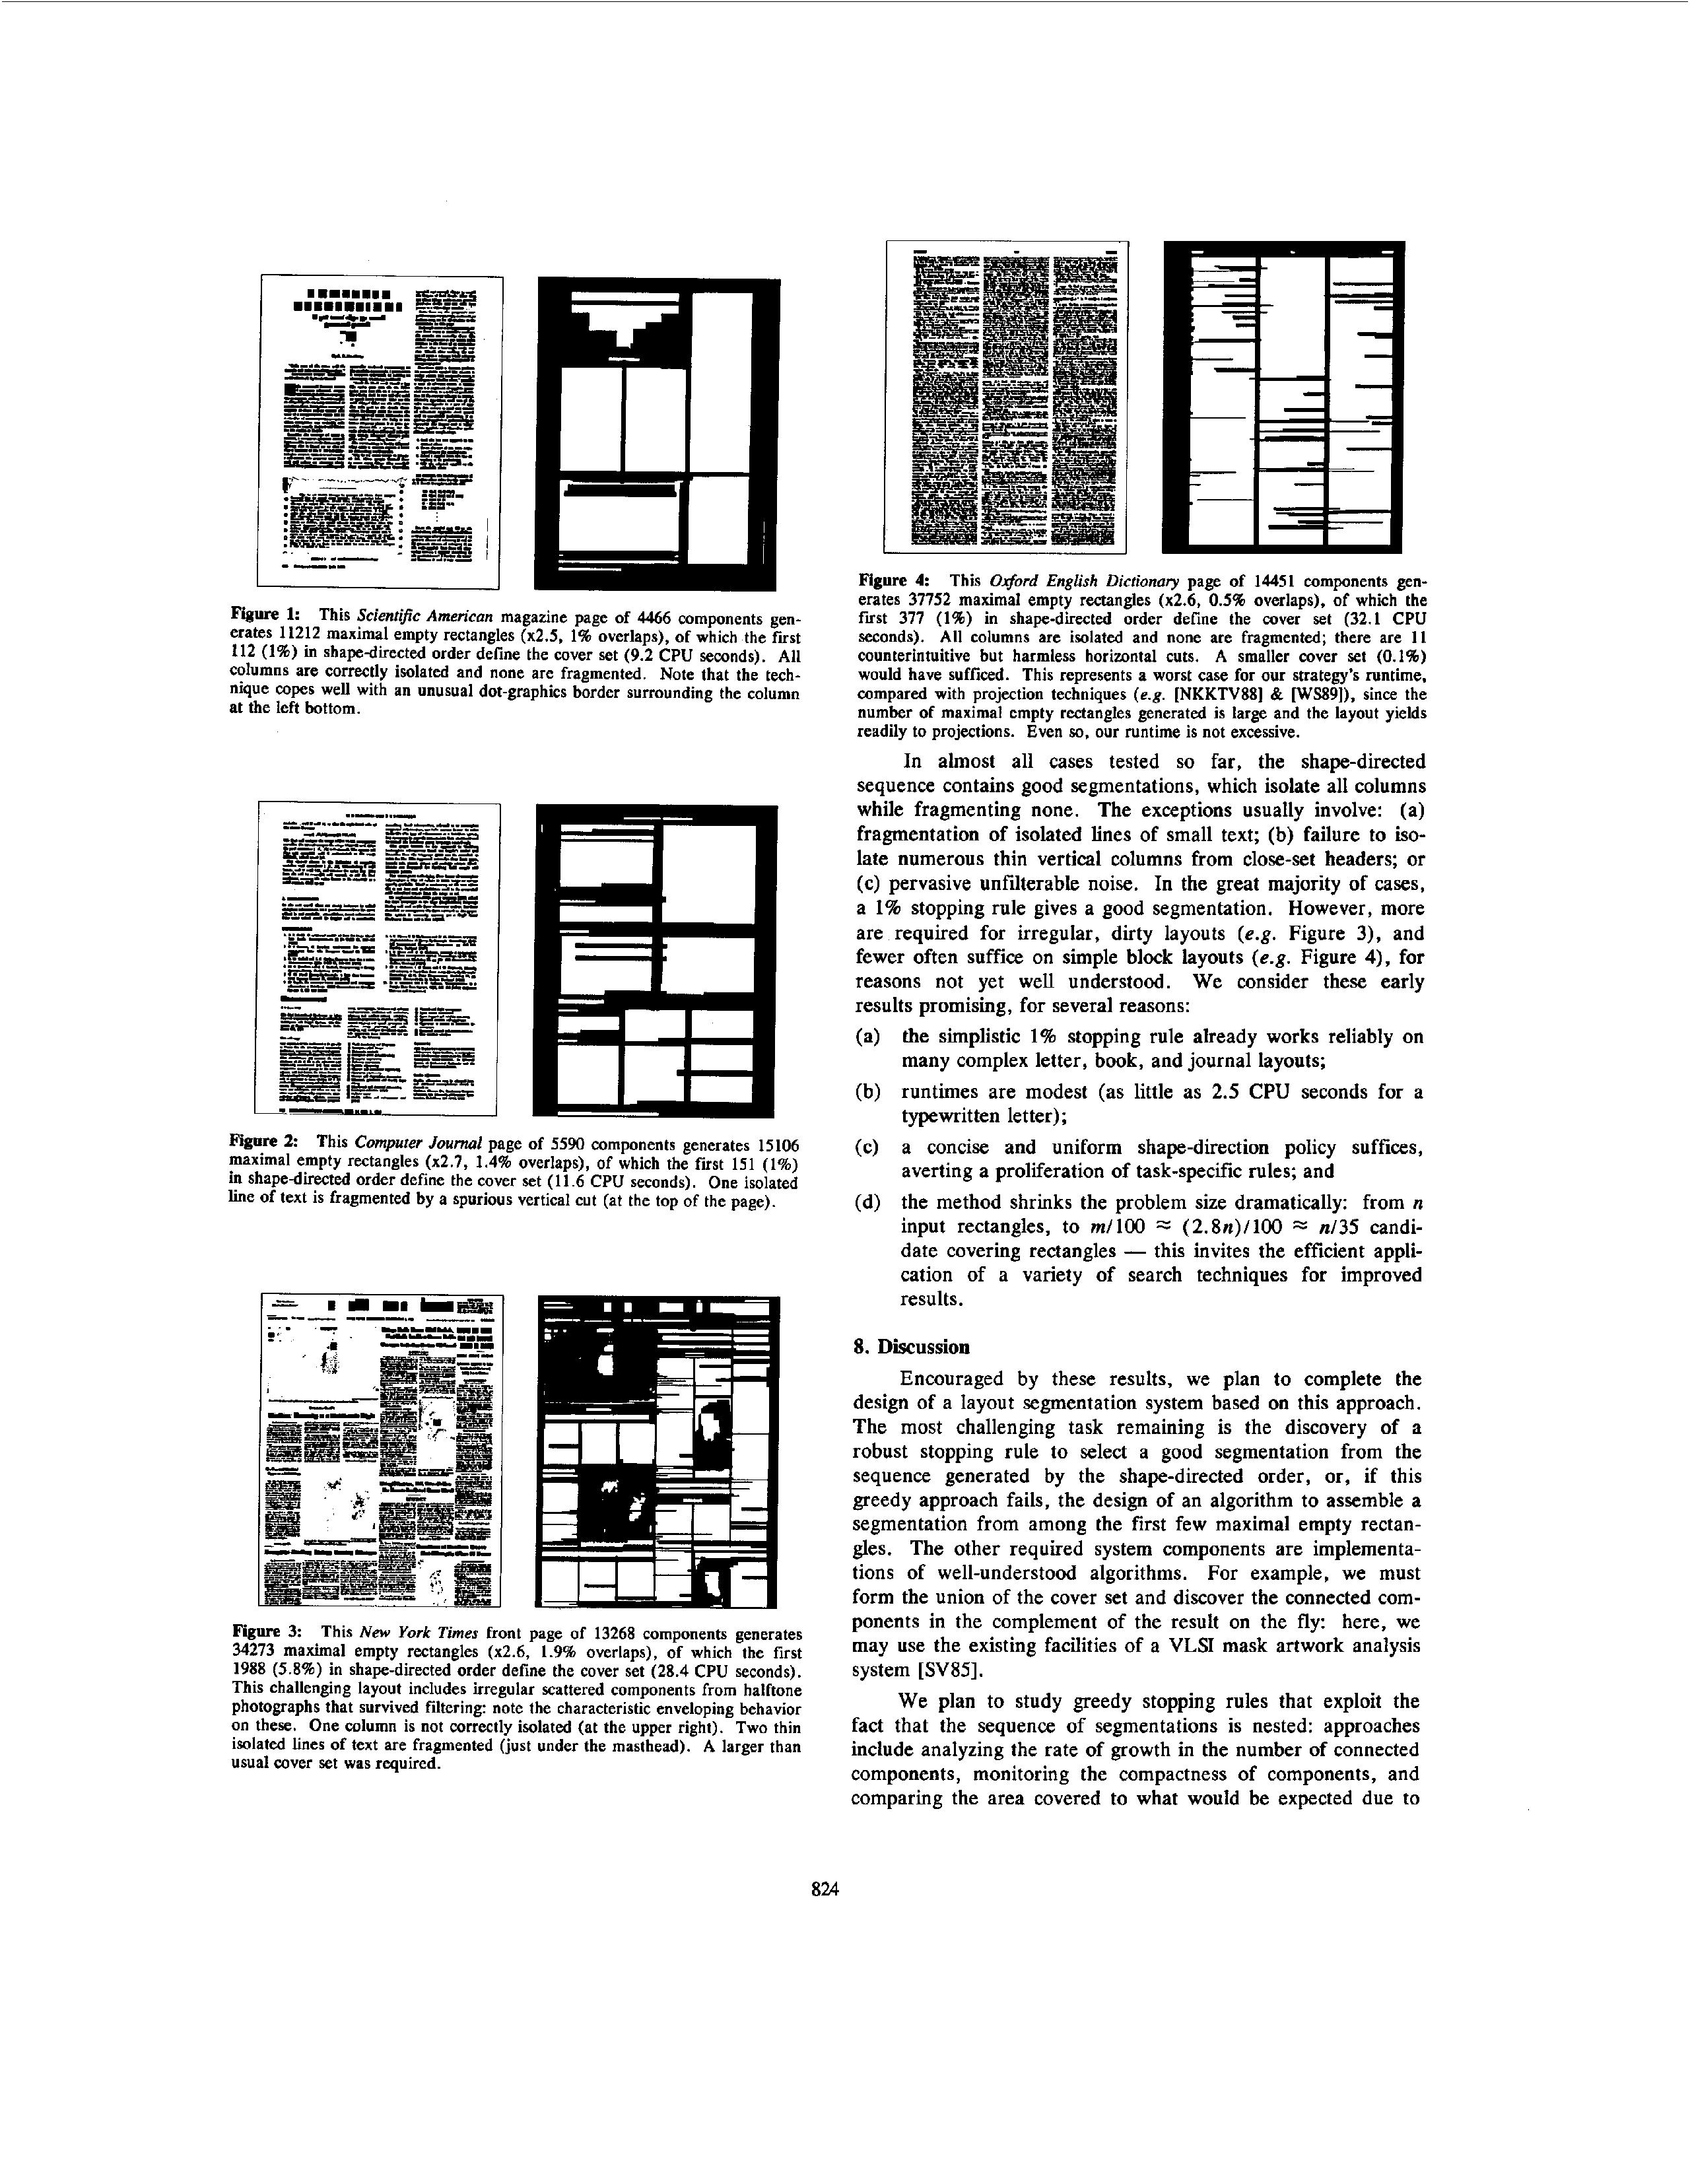
\includegraphics[width = \textwidth]{document1.png}
\end{subfigure}
\hspace*{0.03\textwidth}
\begin{subfigure}{0.47\textwidth}
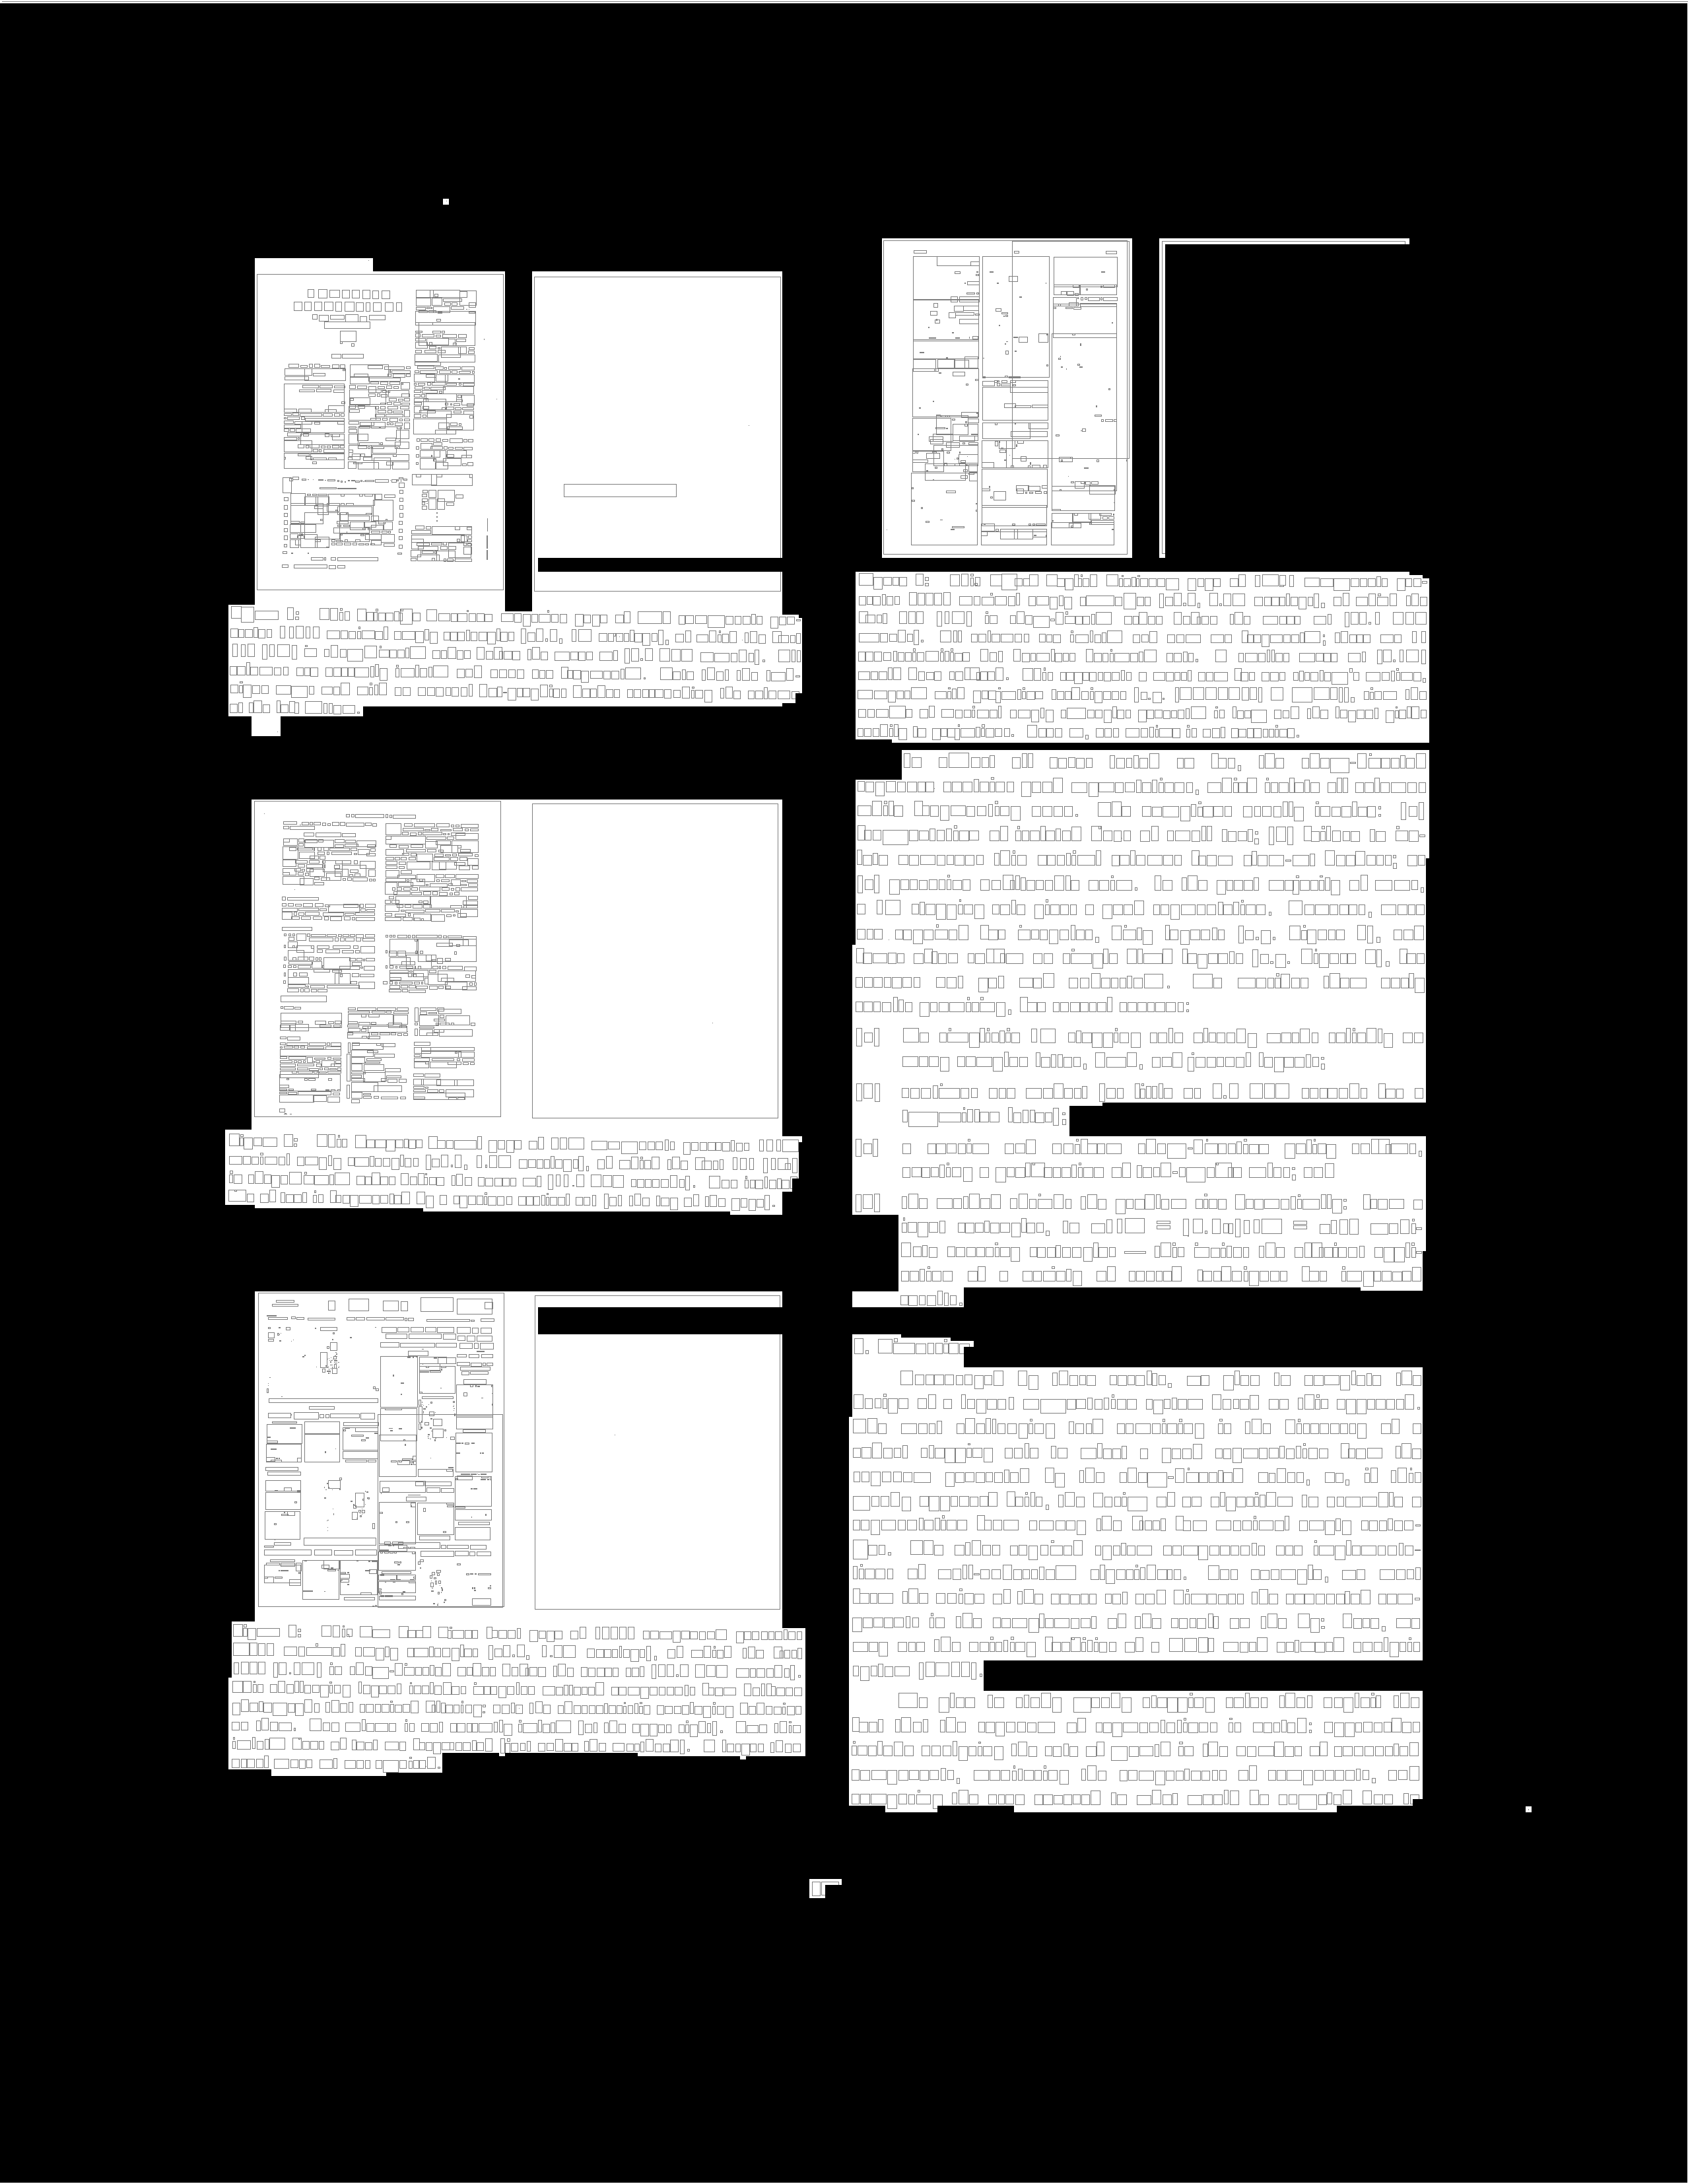
\includegraphics[width = \textwidth]{overlay1.png}
\end{subfigure}
\caption{Left: a typical document. Right: Its generated overlay with MWR enumeration. Rectangles going through figures are a preprocessing
artifact which is corrected further in the processing.}
\label{MWRoverlayEx}
\end{figure}

\section{Algorithm}
The algorithm used to enumerate all the maximum white rectangles in a binary image is described in this section. It is a balanced-tree-based
algorithm, which overall complexity is $\mathcal{O}(n\log(n))$ where $n$ is the number of maximum white rectangles, which itself
amounts to $\mathcal{O}(m^2)$ in the worst case with $m$ the number of black pixels.\\

\subsection{Preprocessing}
For runtime reduction, we use a connected-component reduction pre-processing. Each black connected component is extracted from the original
image, from which we extract a pixel-aligned rectangular frame surrounding it. Only two sides of this frame are kept, the left and top ones.\\

This step reduces every connected component to a 1-pixel thin `$\Gamma$'-like shape, which then can be downsampled with very little loss of
information.
The templates of the connected components are stored for further overlaying after MWR enumeration. With that preprocessing, we achieve a
reduction of the number of black pixels to process by typically 70-80\% before downsampling, that amounts to a total reduction of 85-95\% after
downsampling.\\

A typical 300 dpi letter format document (8.5 Mpx) contains about 1,000,000 black pixels in 10,000 connected components, which is
reduced to a preprocessed image of 1 Mpx with 50,000 - 150,000 black pixels.

\subsection{MWR Enumeration Core Algorithm}

The algorithm sweeps across the document from left to right, processing all black pixels. The pending maximal white rectangles are kept in a
balanced tree structure in which every node represents a rectangle. Such a rectangle is represented by its upper, lower and leftmost bound, until
a black pixel interrupts the rectangle by imposing a right bound.\\

The tree structure is naturally derived from a natural point of view of creating maximal white rectangles sweeping from left to right.
`Thin' white rectangles go from the left margin to the current column in between the already found black pixels. Taller rectangles start at the
right of already processed black pixels. See figure \ref{rectangles}.

\begin{figure}
\centering
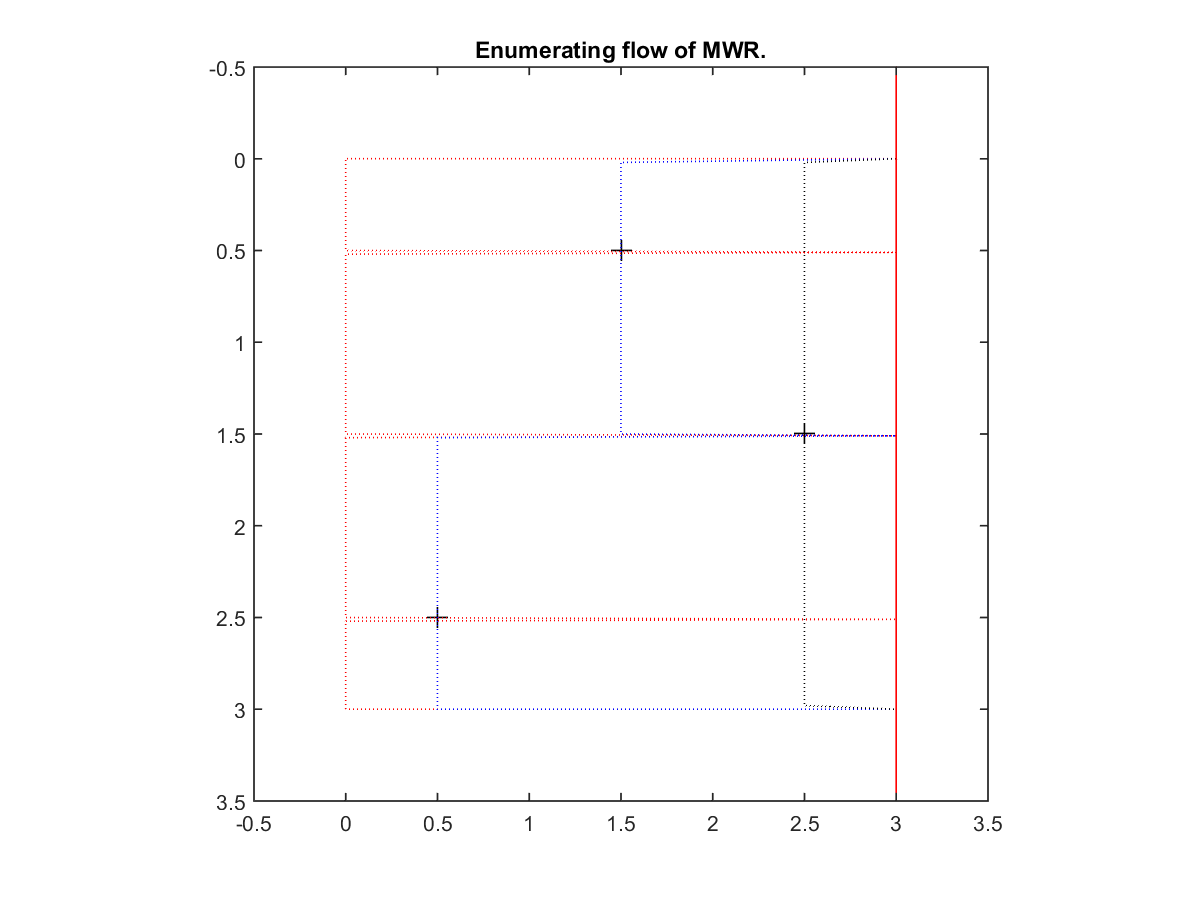
\includegraphics[width = 0.9\textwidth]{rectflow.png}
\caption{State of running MWR enumeration. Solid red: column being processed, Black crosses: black points/pixels. Black dotted: rectangle root of
the tree. Blue dotted: rectangles of depth 1 in the tree. Red dotted: leaves of the tree, corresponding to rectangles going all the way to the
left.}
\label{rectangles}
\end{figure}

The tree is kept balanced with the following invariants:
\begin{itemize}
  \item The leaves of the tree from (left to right) form an uninterrupted partition of the height of the image, all being rectangles starting at
  the left edge.
  \item the root is a rectangle covering the whole height of the paper, with its left edge starting at the last (hence rightmost so far)
  processed black pixel
  \item For any node, the leaves of the subtree below span an exact partition of the height span of the rectangle represented by this node.
  \item For any node, the left bound is larger than the left bound of all rectangles in the subtree below.
\end{itemize}
For the processing step displayed on figure \ref{rectangles}, the rectangle tree would be the following, with the syntax
\verb+([top,bottom],left)+ for a running rectangle.\\

\begin{verbatim}
                            ([0,3], 2.5)
                           /            \
             ([0,1.5], 1.5)             ([1.5,3], 0.5)
           /              \            /             \
     ([0,0.5], 0)  ([0.5,1.5],0) ([1.5,2.5],0)    ([2.5,3],0)
\end{verbatim}

The invariants described above are preserved by the following process for integrating a new black pixel:
\begin{itemize}
  \item Find the lowest node being split if the vertical direction by this black point. Discard all the nodes that are split as finished MWRs.
  \item split the tree along the split node and its fathers (that are all split as well). A rebalancing operation not described here ensures that
  the depth does not increase dramatically during these operation.
  \item Merge the two trees generated by the previous step under a new root, a rectangle starting a the current black pixel and spanning the
  whole height.
\end{itemize}

\subsection{Implementation}
It is to be noted that the algorithm described above processes ponctual black dots in a continuous 2D space. Optimizations can be done when we
know black dots are actually 1-px wide and necessarily lie on a grid. Otherwise, we just need to discard 1-unit wide rectangles as being
nonexistent (in between contiguous black pixels).\\

For performance, the algorithm was implemented in the Java language, achieving a runtime of about 8 seconds for a typical document.

\section{Post-processing}
The process allows to successively discard maximal white rectangles in a binary layout. This rectangles are immediately pushed in a priority
queue which keeps them sorted by a user-defined metric.\\
Empirically, the rectangles that best separate the logical block without going through them are the large rectangles with a large aspect ratio,
such as ones running between columns or cutting in between two paragraphs, or between a figure and its caption. For that purpose, the following
classifying metric was empirically developed by Henri S. Baird, and is the one we used in this project with encouraging results. The ceiling of
aspect ratio to 16 is somehow arbitrary but allows to avoid growing the score of -for instance- very thin rectangles that run in between
characters.
\[
\mathrm{score} = \mathrm{area} \times \log(\min(\mathrm{aspect ratio}, 16))
\]
Finally, a certain percentage has to be chosen to construct the image layout. In this project, we have used the value of 1\%, providing typical
results as shown in figure \ref{MWRoverlayEx}. Typically our preprocessed images contain about 15,000 MWR, and between 100-200 MWR is a good
quantity to determine the block-by-block layout without separating lines with smaller rectangles.\\

After this MWR layout processing, logical components are isolated and can be analyzed either independently or together to determine their nature
and logical connections, which is done in the following steps of the project.

\end{document}
